\documentclass[10pt]{article}
\usepackage[margin=3cm]{geometry}
\usepackage{amssymb}
\usepackage{verbatim}
\usepackage{graphicx}
\usepackage{amsmath}
\title{\bfseries\Huge Bram van den Akker}

\date{}
\begin{document}
\title{Convergence between high performance and embedded systems}
\author{Abe Wiersma, Bram van den Akker}
\date{\today}
\maketitle
\newpage

\section{Introduction}
In this short literature study we will be taking a look at both high performance and embedded system, their difference, their growth and the convergence between the two of them. 

\subsection{Embedded systems}
For a computer system to be specified as an embedded system it has to have a dedicated function. Example embedded systems range from mp3 players, smart phones, anti-lock braking systems in a car, MRI and a rocket guidance computer (The first recognizable embedded system actually was the Apollo Guidance Computer). 

\begin{figure}[h]
  \centering
    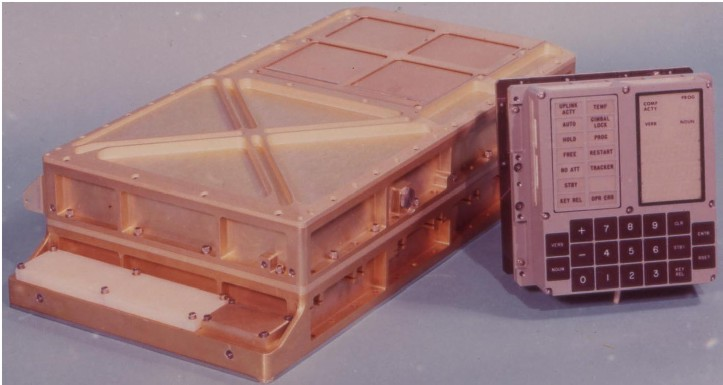
\includegraphics[width=\textwidth]{apollo.jpg}
  \caption {Apollo Guidance Computer by Charles Stark Draper.}
\end{figure}

Embedded systems exist in very different forms. An embedded system can exist without an user interface (anti break system) or have a complex full user interface (smart phones). Opposing the desktop market were computers are limited to a few CPU architectures an embedded system can use many different CPU architectures, using the architecture optimized for the purpose. To be able to perform certain tasks peripherals like sensors, I/O ports and ethernet can be added to the system. Many embedded systems can be acquired for low pricing due to their mass production and are very power efficient. 

\subsection{High performance systems}
Higher performance systems are powerful multi-purpose computer systems which can be used in a wide series of task. Common high performance computer systems are servers, desktop PC's and supercomputer. High performance computer systems are commonly expensive and consume high amounts of energy. High performance computer systems can be used for i.e. large simulations, rendering complex computer graphics and many day to day computing task.

Many high performance computer systems use both graphics processing units(GPU) and central processing units (CPU) for their computations. GPU's are able to preform a single operation to multiple values at the same time, which is a great advantage for large computational tasks.


\end{document}